\documentclass[oneside]{usachtesis} %%clase para tesis usach
\usepackage[cm]{sfmath}

%%package para bibliografía
\usepackage{natbib}

\usepackage{mhchem}

\usepackage{fancyhdr}

\usepackage{titlesec}

\usepackage{gensymb}

\usepackage{subcaption}

\usepackage{pgfplots}
\usepackage{pgfplotstable}
\usetikzlibrary{external}
%\usepgfplotslibrary{external}
\tikzexternalize[prefix=Imagenes/tikzext/]

\usetikzlibrary{positioning}

\newcommand{\plotwidth}{0.3\textwidth}
\newcommand{\plotscale}{0.8}

\pgfplotsset{
	compat=1.15,
	CVStyle/.style={
		title=Voltametría Cíclica,
		domain=-0.8:0.8,
		xtick distance=0.4,
		minor tick num=1,
		ylabel={Densidad de corriente [A/g]},
		xlabel={Voltaje [V]},
		every axis legend/.append style={
			font=\tiny,
			at={(0.98,0.02)},
			anchor=south east,
		},
		legend entries={25mV/s,50mV/s,100mV/s,200mV/s,400mV/s},
		cycle list name=exotic,
		no markers,
	},
	SCStyle/.style={
		title=Capacidad Específica,
		domain=25:400,
		ylabel={Capacidad específica [F/g]},
		xlabel={Velocidad de barrido [mV/s]},
		every axis legend/.append style={
			font=\tiny,
			at={(0.98,0.98)},
			anchor=north east,
		},
		legend entries={Antes, Después},
		cycle list name=exotic,
	},
	EISStyle/.style={
		title=Espectro de impedancia electroquímica,
		domain=0:50,
		ylabel={-Z imag [Ohm]},
		xlabel={Z real [Ohm]},
		cycle list name=exotic,	
	},
	CCDStyle/.style={
		title=Carga y descarga cíclica,
		ylabel={Voltaje [V]},
		xlabel={Tiempo [s]},
		cycle list name=exotic,
		mark size = 0.2pt,
		line width = 0.1pt,
		only markers,
		every axis legend/.append style={
			font=\tiny,
			at={(0.98,0.02)},
			anchor=south east,
		},
		legend entries={Primeros ciclos, Últimos ciclos},
	},
}


\fancypagestyle{plain}{%
	\fancyhf{} % clear all header and footer fields
	\fancyhead{} % clear all header fields
	\fancyfoot{} % clear all footer fields
	\fancyfoot[RO]{\thepage}
	\renewcommand{\headrulewidth}{0pt}
	\renewcommand{\footrulewidth}{0pt}
}
\pagestyle{plain}

\titleformat{\chapter}
{\normalfont\bfseries}{\thechapter}{11pt}{}

\titleformat{\section}
{\normalfont\bfseries}{\thesection}{10pt}{}

\titleformat{\subsection}
{\normalfont}{\thesubsection}{1em}{}

\titleformat{\subsubsection}
{\normalfont}{\thesubsubsection}{1em}{}


%\sansmath % Enable sans-serif math for rest of document

\makeindex
\setcounter{tocdepth}{1}

\graphicspath{{Imagenes/}}

\newcommand*\circled[1]{%
	\tikz[baseline=-5]{\node[draw,circle,inner sep=1pt] {#1};}
	}

%============================================================
%===================Comienzo del documento===================
%============================================================
\begin{document}
%%PORTADA						
 \title{Síntesis de Grafeno por medios químicos y construcción de supercondensadores basados en grafeno}
 \author{Carlos Javier Eugenio Herrera}
 \facultad{CIENCIA}
 \departamento{FÍSICA}
 \profesorguia{DINESH PRATAP SINGH}
 \tituloprofesional{Ingeniero Físico}
 \anolol{2017}
 
\begin{titlepage}
	\maketitle
\end{titlepage}

\newpage
\mbox{}
\thispagestyle{empty}
\pagenumbering{roman}

%%DERECHOS DE AUTOR
\derechosdeautor

%%HOJA DE CALIFICACIONES
\newpage
\thispagestyle{empty}

%%DEDICATORIA
\newpage
\chapter*{}
\begin{flushright}
\textit{Dedicado a...}
\end{flushright}
\newpage

%%AGRADECIMIENTOS(OPTATIVA)
\chapter*{Agradecimientos}

%%TABLA DE CONTENIDOS
\newpage
\tableofcontents
\newpage
\newrgbcolor{xdxdff}{0.49 0.49 1}
\newrgbcolor{ffqqtt}{1 0 0.2}
\psset{xunit=1.0cm,yunit=1.0cm,algebraic=true,dotstyle=*,dotsize=3pt
0,linewidth=0.8pt,arrowsize=3pt 2,arrowinset=0.25}

%%ÍNDICE DE TABLAS
\newpage
\listoftables
\newrgbcolor{xdxdff}{0.49 0.49 1}
\newrgbcolor{ffqqtt}{1 0 0.2}
\psset{xunit=1.0cm,yunit=1.0cm,algebraic=true,dotstyle=*,dotsize=3pt
	0,linewidth=0.8pt,arrowsize=3pt 2,arrowinset=0.25}

%%INDICE DE ILUSTRACIONES
\newpage
\listoffigures
\newrgbcolor{xdxdff}{0.49 0.49 1}
\newrgbcolor{ffqqtt}{1 0 0.2}
\psset{xunit=1.0cm,yunit=1.0cm,algebraic=true,dotstyle=*,dotsize=3pt
0,linewidth=0.8pt,arrowsize=3pt 2,arrowinset=0.25}

%%RESUMEN
\newpage
%%RESUMEN
\chapter*{Resumen}
\addcontentsline{toc}{chapter}{Resumen}
asdasdasdasddddddddddddddddddddddd

%%INTRODUCCIÓN
\newpage
%%%INTRODUCCIÓN GENERAL%%%
\chapter*{Introducción}
\addcontentsline{toc}{chapter}{Introducción}
\section*{Objetivos}
\addcontentsline{toc}{section}{Objetivos}
\subsection*{Objetivo general}
\begin{itemize}
	\item Sintetizar óxido de grafeno reducido, para su utilización en electrodos de supercondensadores.
\end{itemize}
\subsection*{Objetivos específicos}
\begin{itemize}
	\item Sintetizar óxido de grafeno (GO), a partir de grafito natural mediante un proceso químico; para su posterior reducción y obtención de óxido reducido de grafeno (rGO).
	\item Fabricar electrodos de óxido de grafeno reducido con diferentes métodos, para su posterior caracterización electroquímica.
	\item Diseñar y construir una celda de prueba de supercondensadores para estudiar el desempeño de diferentes electrodos fabricados.
	\item Elaborar una metodología de medición electroquímica para cuantificar y comparar el desempeño de los diferentes electrodos fabricados. 
\end{itemize}

\newpage
\section*{Nanociencia}
\addcontentsline{toc}{section}{Nanociencia}
El prefijo nano deriva del griego $\nu \tilde{\alpha} \nu o \varsigma$, que significa literalmente ``enano''. En el sistema internacional de unidades, el prefijo nano representa un factor de $\mathrm{10^{-9}}$, o una mil millonésima parte. Al añadir este prefijo a la unidad de longitud, obtenemos ``nanómetro'' (nm), o una mil millonésima parte de un metro. Así la nanotecnología es, a grandes rasgos, la ciencia, tecnología, e ingeniería que trata sistemas en el rango aproximado de 1-100 nanómetros \citep{Haick2013,Gressler2013}. Esta definición es práctica pero resulta poco precisa, un nanomaterial debe ser considerado como tal cuando comienza a exhibir un cambio en sus propiedades debido a la reducción de sus dimensiones, ésta es propia de cada material y por tanto no puede ser estandarizada. Se ha de tener claro en qué rango de dimensiones se encuentra la escala nanométrica, los seres humanos estamos acostumbrados a escalas grandes, se nos hace fácil entender las comparaciones de kilómetros con metros, o milímetros con metros, pero al reducir el tamaño a micrómetros o nanómetros nos cuesta, pues son escalas que escapan a nuestros sentidos. Para ponerlo en perspectiva, un nanómetro es a un metro, como un metro es a un millón de kilómetros. La figura \ref{fig:scale} muestra una escala de tamaños con varios ejemplos desde la escala humana hasta la atómica.

\begin{figure}[h!]
	\centering
	\fbox{
		\includegraphics[width=\textwidth]{scale.pdf}
	}
	\caption[Comparativa de ódenes de magnitud desde metros hasta picometros]{Comparativa de órdenes de magnitud. De izquierda a derecha: Escala humana, 1-2 m. Insectos, 10 cm - 1 mm. Glóbulos rojos, 6 $\mathrm{\mu}$m. Longitud de onda de luz visible, 780-380 nm. Transistores en un microprocesador, 100 - 10 nm. Doble hélice de ADN, 2 nm. Radio atómico de un átomo de helio, 31 pm.}
\label{fig:scale}
\end{figure}

La idea de la nanotecnología fue vislumbrada, entre otros, por el físico Richard Feynman y expuesta en su charla \emph{``There is plenty room at the bottom''} \citep{Feynman1960}. Feynman plantea que no existen barreras físicas que impidan manipular sistemas nanométricos, moléculas, o incluso átomos. La era moderna de la nanotecnología comienza con el desarrollo del microscopio de efecto túnel por Binning y Rohrer en 1981 \citep{Binnig1982}, que les hizo ganar el Premio Nobel de Física en el año 1986. Un microscopio de efecto túnel (STM por sus siglas en inglés \emph{Scanning Tunneling Microscope}), puede superar resoluciones de 0,1 nm de resolución lateral, 0,01 nm en profundidad, y trabajar en variadas condiciones, sin necesidad de alto vacío o bajas temperaturas. Además de poder resolver átomos, el STM también puede manipularlos \citep{Chen2008}.

Una forma simple de clasificar los nanomateriales surge del número de dimensiones del material que no están en la nanoescala (ver figura \ref{fig:carbon_allotropes}). Un material que no posee ninguna dimensión en la nanoescala (material \emph{bulk}), se denomina material 3D y no  se considera un nanomaterial\footnote{A veces se les llama nanomateriales 3D a materiales formados por nanomateriales (2D, 1D, o 0D), que forman estructuras tridimensionales macroscópicas y muestran propiedades de nanomateriales, como por ejemplo, los aerogeles.}. Si una dimensión del material está en la nanoescala, se habla de material 2D, análogamente, con dos dimensiones en la nanoescala se trata de un nanomaterial 1D, y por último, si todas las dimensiones están en la nanoescala se denomina nanomaterial 0D.

\begin{figure}
	\centering
	\begin{subfigure}[b]{0.2\textwidth}
		\includegraphics[width=\textwidth]{graphite_structure.pdf}
		\caption{}
		\label{fig:graphite_struct}
	\end{subfigure}
	\begin{subfigure}[b]{0.2\textwidth}
		\includegraphics[width=\textwidth]{graphite_image.jpg}
		\caption{}
		\label{fig:graphite_image}
	\end{subfigure}
	\begin{subfigure}[b]{0.2\textwidth}
		\includegraphics[width=\textwidth]{graphene_structure.pdf}
		\caption{}
		\label{fig:graphene_struct}
	\end{subfigure}
	\begin{subfigure}[b]{0.2\textwidth}
		\includegraphics[width=\textwidth]{graphene_image.jpg}
		\caption{}
		\label{fig:graphene_image}
	\end{subfigure}
\\
	\begin{subfigure}[b]{0.2\textwidth}
		\includegraphics[width=\textwidth]{cnt_structure.pdf}
		\caption{}
		\label{fig:cnt_struct}
	\end{subfigure}
	\begin{subfigure}[b]{0.2\textwidth}
		\includegraphics[width=\textwidth]{cnt_image.png}
		\caption{}
		\label{fig:cnt_image}
	\end{subfigure}
	\begin{subfigure}[b]{0.2\textwidth}
		\includegraphics[width=\textwidth]{fullerene_structure.pdf}
		\caption{}
		\label{fig:fullerene_structure}
	\end{subfigure}
	\begin{subfigure}[b]{0.2\textwidth}
		\includegraphics[width=\textwidth]{fullerene_image.jpg}
		\caption{}
		\label{fig:fullerene_image}
	\end{subfigure}
	\caption[Alótropos del carbono mostrando las diferentes dimensionalidades de los nanomateriales]{Estructuras e imágenes de varios alótropos del carbono como ejemplos de la dimensionalidad de los nanomateriales:  \subref{fig:graphite_struct} y \subref{fig:graphite_image} grafito natural, un material 3D. \subref{fig:graphene_struct} y \subref{fig:graphene_image} grafeno, imagen de microscopía de efecto túnel (Frank Trixler, LMU/CeNS: Organic Semiconductor Group), un material 2D. \subref{fig:cnt_struct} y \subref{fig:cnt_image} nanotubo de carbono, imagen SEM de un dispositivo para medir diferentes propiedades del nanotubo (Pavlos Apostolidis, London Centre for Nanotechnology, Department of Physics \& Astronomy), un material 1D. \subref{fig:fullerene_structure} y \subref{fig:fullerene_image} fullereno, imagen TEM de fullerenos C80 funcionalizados dentro de un nanotubo de carbono \citep{Gimenez2011}, un material 0D.}
	\label{fig:carbon_allotropes}
\end{figure}

\subsection*{La física de sistemas nanométricos}
Al reducir las dimensiones a escalas nanométricas, surgen efectos de confinamiento cuántico, pues se restringe el movimiento de los electrones en el material. Esto conlleva a la discretización de los niveles de energía de los electrones y al cambio de la densidad de estados del material al tratarse de semiconductores (figura \ref{fig:DoE}). Dependiendo de cuantas dimensiones son llevadas a la nanoescala, es como se ve afectada la densidad de estados.

\begin{figure}[h!]
	\centering
	\fbox{
		\includegraphics[width=0.6\textwidth]{DoE.pdf}
	}
	\caption[Densidad de estados en diferentes dimensionalidades]{Densidad de estados en diferentes dimensiones. Para materiales 3D (no nanoestructurados), la densidad de estados es continua. En nanomateriales 2D, la densidad de estado forma escalones. Para materiales 1D, ésta es discontinua, y para nanomateriales 0D es completamente discreta. }
	\label{fig:DoE}
\end{figure}

Por otra parte, si un determinado volumen es dividido en partículas más pequeñas, el área superficial aumenta. Por ejemplo, como se muestra en la secuencia de la figura \ref{fig:area_cubes}, el volumen total, o cantidad de material en cada división no cambia, pero el área superficial se duplica \footnotemark, siguiendo está lógica, al fragmentar un cubo de lado 1 cm a cubos de lado 100 nm, el área total habrá aumentado 100.000 veces. El aumento del área superficial aumenta la reactividad del material, ya que hay más lugar para reacciones químicas. Otra forma de verlo es considerar la proporción de átomos en la superficie, con la cantidad de átomos al interior de una partícula. En la figura \ref{fig:graph_nanocube} se aprecia como aumenta esta proporción al disminuir el tamaño de una nanopartícula.

\footnotetext{Si en la secuencia de la figura \ref{fig:area_cubes} el cubo más grande tiene lado $l$, su área superficial es $6 \times l^2$, en la primera división, el lado de cada cubo es $l/2$ y el área de cada uno es $6\left( l/2\right)^2$, que en total hacen $6\left(l/2\right)^2\times 8$, en la segunda división el área total es $6\left(l/4\right)^2\times 8 \times 8$, así, en la n-ésima división el área es $6l^2 \left(1/2^n\right)^2\times 8^n$ o $6l^2 \times 2^n$. Así, el área superficial se dobla con cada división.}

\begin{figure}[h!]
	\centering
	\begin{subfigure}{\textwidth}
		\fbox{
			\includegraphics[width=\textwidth]{area_cubes.pdf}
			}
		\caption[Subdivisiones de un cubo demostrando el aumento de área superficial total]{Subdivisiones de un cubo demostrando el aumento de área superficial total.}
		\label{fig:area_cubes}
	\end{subfigure}
	\begin{subfigure}{\textwidth}
			\begin{tikzpicture}[]
				\begin{axis}[
				width=\textwidth,
				height=\axisdefaultheight,
				change x base,
				cycle list name=colorbrewer-RYB,
				width = \textwidth,
				ylabel={Proporción de átomos},
				yticklabel=\pgfmathparse{100*\tick}\pgfmathprintnumber{\pgfmathresult}\,\%,
				xlabel={Tamaño de partícula},
				x unit=m,
				x SI prefix=nano,
				legend entries={En la superficie, Dentro de la partícula}]	
				\addplot table [x expr = \thisrow{l}, y expr=\thisrow{surf}] {./Data/nanocube.txt};
				\addplot table [x expr = \thisrow{l}, y expr=\thisrow{bulk}] {./Data/nanocube.txt};
				\end{axis}
			\end{tikzpicture}
			\caption{Proporción de átomos en la superficie y dentro de cada nanopartícula en relación a su tamaño.}
			\label{fig:graph_nanocube}
	\end{subfigure}
	\caption[Aumento de área superficial y proporción de átomos en superficie al disminuir el tamaño de las nanopartículas]{\subref{fig:area_cubes}Si se subdivide un cubo de 1 cm de lado hasta tener cubos de 100 nm de lado, el área superficial total pasaría de 6 $\mathrm{cm^2}$ a 60 $\mathrm{m^2}$. En este caso, el lado de cada cubo disminuye 100.000 veces, aumentando el área superficial total por el mismo factor.}
\end{figure}

\subsection*{Síntesis de nanomateriales}
Dependiendo de la vía de aproximación a la nanoescala, se distinguen dos formas de síntesis. Por un lado, si partimos de la forma macroscópica de un material y de algún modo se reducen sus dimensiones hacia la nanoescala, se habla de un proceso \textit{top-down}, por ejemplo la exfoliación del grafito (\textit{bulk material}) para obtener grafeno (nanomaterial) \citep{Novoselov2004}.  Por otro lado, sintetizar un nanomaterial a partir de átomos o moléculas es un proceso \textit{bottom-up}, un ejemplo es la síntesis de nanopartículas de oro a partir de un precursor como el ácido tetracloroaúrico \citep{Daniel2004}.

\subsection*{Caracterización de nanomateriales}
Los nanomateriales son caracterizados usando técnicas comunes que se utilizarían para materiales no nanoestructurados dependiendo de las características que se deseen estudiar.




%%CAPÍTULOS
\newpage
\pagenumbering{arabic}
%\chapter{Nanomateriales basados en carbono}
%	%\chapter{Nanomateriales} //is included in Marco teorico file
\noindent
\rule{\linewidth}{1 pt}
\begin{flushright}
	\begin{quotation}
		\small{
			\textit{``There’s Plenty of Room at the Bottom.''}}
	\end{quotation}
	\bf{Richard Feymann}
\end{flushright}
\noindent
\rule{\linewidth}{1 pt}\\
\vfill
\section{Nanomateriales}
%TODO ejemplos de longitudes características
Generalmente la denominación nano es atribuida a materiales en que algunas de sus dimensiones estén en la escala nanométrica, entre 1-100 nm \citep{Gressler2013}. Ésta definición es práctica pero poco precisa en el sentido que algunos materiales exhiben características propias de los nanomateriales fuera de este rango ($>$ 100 nm). Por esta razón es preferible hablar de nanomateriales cuando se comienzan a mostrar éstas nuevas características. El momento en cual aparecen estos cambios, es propia de cada material, y está asociado a alguna longitud característica de éste. Algunos ejemplos, el camino libre medio de un electrón,

\section{Síntesis}
Dependiendo de la vía de aproximación a la nanoescala, se distinguen dos formas de síntesis, por un lado, si partimos de la forma macro de un material y de algún modo se reducen sus dimensiones hacia la nanoescala, se habla de un proceso \textit{top-down}. Por ejemplo, la exfoliación del grafito (\textit{bulk material}) para obtener grafeno (nanomaterial) \citep{Novoselov2004}.  Por otro lado, sintetizar un nanomaterial a partir de átomos o moléculas es un proceso \textit{bottom-up}, un ejemplo es la síntesis de nanopartículas de oro a partir de un precursor como el ácido tetracloroaúrico \citep{Daniel2004}.

\section{Caracterización}


\section{Aplicaciones}


\section*{Grafeno}
\addcontentsline{toc}{section}{Grafeno}
	%\chapter{Grafeno}
\noindent
\rule{\linewidth}{1 pt}
\begin{flushright}
	\begin{quotation}
		\small{
			\textit{``What is important about graphene is the new physics it has delivered.''}}
	\end{quotation}
	\bf{Andre Geim}
\end{flushright}
\noindent
\rule{\linewidth}{1 pt}\\
\vfill

\section{Óxido reducido de grafeno (RGO)}
Para producir grapfeno que sea utilizable en aplicaciones que requieran grandes cantidades de este, como recubrimientos, baterías, supercondensadores,etc. se hace necesario buscar nuevos métodos que entreguen volúmenes grandes de material utilizable, y a su vez, de bajo costo, e idealmente amigable con el medio ambiente. 
\section{Síntesis}

\section{Aplicaciones}
\section*{Supercondensadores}
\addcontentsline{toc}{section}{Supercondensadores}
	%\chapter{Supercondensadores}
Almacenar energía eléctrica es uno de los mayores problemas a la hora de diseñar sistemas electrónicos móviles o estacionarios, los requerimientos varían de acuerdo a las necesidades de cada uno, en general es una competencia entre la densidad de energía (cuánta energía se puede almacenar) y la densidad de potencia (que tan rápido puede ser entregada la energía almacenada). Para poner en perspectiva las tecnologías de almacenamiento de energía, existe el diagrama de Ragone (ver figura \ref{fig:ragone}). Las celdas de combustible de hidrógeno (\textit{Fuel Cells}), entregan la mayor densidad de energía, pero son complicadas debido a las dificultades que presenta el almacenar hidrógeno \citep{Hadjipaschalis2009}. Mientras que las baterías poseen mayor densidad de potencia, pierden capacidad con los ciclos de carga y descarga rápidamente. Los supercondensadores van un paso más allá, aumentado la densidad de potencia y aportando mayor vida útil, entregando una nueva posibilidad a la hora de diseñar sistemas eléctricos, ya sea como fuente de energía por sí mismo, o en sistemas híbridos combinados con otras tecnologías \citep{Thounthong2009}.\\
La densidad de energía de un supercondensador comparada a la de un condensador convencional es varios órdenes de magnitud superior, a modo de comparación, generalmente se utilizan microfaradios (10$^{-6}$ Faradios), para medir la capacidad de un condensador convencional, mientras que en un supercondensador es común ver capacidades de decenas o centenas de Faradios.


\begin{figure}
	\centering
	\fbox{
		\includegraphics[width = 0.7\textwidth]{ragone.pdf}
	}
	\caption[Diagrama de Ragone, diferentes tecnologías de almacenamiento de energía]{El diagrama de Ragone compara diferentes tecnologías de almacenamiento de energía de acuerdo a su densidad de potencia y densidad de energía.}
	\label{fig:ragone}
\end{figure}

\subsection{El condensador ideal}
Generalmente un condensador se modela a través de dos placas paralelas separadas por un dieléctrico. Éste es definido por su capacitancia, la que refleja, \emph{grosso modo}, su capacidad de almacenar energía. Del modelo de placas paralelas se desprende la definición de capacitancia, $C$, como la razón entre la magnitud de carga en cada placa $Q$ y el voltaje entre los terminales $V$:

\begin{equation}
	C = \frac{Q}{V}
\end{equation}

La magnitud C es constante y depende de la construcción del condensador. Para fines prácticos, el condensador ideal como componente electrónico es modelado por la ecuación que relaciona la corriente\footnote{En estricto rigor, no hay corriente en el condensador, pues los electrones no ``saltan'' de una placa a otra, sólo se acumulan en una y se remueven en la otra, aparentando una corriente a través del dispositivo. La corriente en el condensador, es más bien una corriente de desplazamiento, pues es el campo eléctrico el que varía en el condensador.} con el voltaje entre los terminales del dispositivo. Considerando que $i = dq/dt$, entonces:

\begin{equation}
	i(t) = C \frac{dv(t)}{dt}.
\end{equation}
Esto quiere decir que la corriente es proporcional a la variación del voltaje en el tiempo.
En el caso de un proceso de carga y descarga a corriente constante, el voltaje variará linealmente, como lo muestra el gráfico de la figura \ref{fig:plot:charge-discharge_ideal_cap}.

\begin{figure}
	\centering
	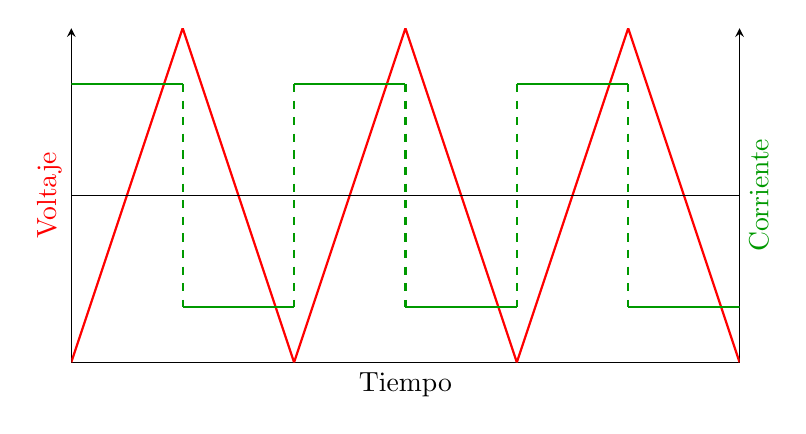
\begin{tikzpicture}
	% let both axes use the same layers
	\pgfplotsset{set layers, 	width=0.7\textwidth, height = 0.35\textwidth}
	
	\begin{axis}[
	scale only axis,
	axis y line=left, % the ’*’ avoids arrow heads
	axis x line*=bottom,
	xlabel=Tiempo,
	ylabel={\color{red} Voltaje},
	no markers,
	xmin=0,
	xmax=6,
	cycle list name=exotic,
	ticks=none,
	]
		\addplot [red, thick] table {
			A B
			%charge
			0 -1
			1  1
			
			2 -1
			3  1
			
			4 -1
			5  1
			
			%discharge
			1  1			
			2 -1
			
			3  1
			4 -1
			
			5  1
			6 -1
		};	
	\end{axis}
	\begin{axis}[
	scale only axis,
	axis y line=right,
	axis x line=none,
	ylabel={\color{green!60!black} Corriente},
	ymin = -1.5,
	ymax = 1.5,
	xmin = 0,
	xmax = 6,
	no markers,
	ticks=none,
	]
		\addplot [green!60!black, thick] table {
			A B
			0  1
			1  1
			
			1 -1
			2 -1
			
			2  1
			3  1
			
			3 -1
			4 -1
			
			4  1
			5  1
			
			5 -1
			6 -1	
		};
		\addplot [green!60!black, thick, dashed] table {
			A B
			1  1
			1 -1

			2  1
			2 -1
			
			3  1
			3 -1
			
			4  1
			4 -1
			
			5  1
			5 -1
		};
		\addplot [black] table {
			0  0
			6  0
		};
	\end{axis}
	\end{tikzpicture}
	\caption[Carga y descarga de un condensador ideal a corriente constante]{Carga y descarga de un condensador ideal a corriente constante.}
	\label{fig:plot:charge-discharge_ideal_cap}
\end{figure}

\subsection{El condensador real}
%TODO agregar electrolito no acuoso
Un condensador ideal almacenaría una cierta cantidad de energía al cargarse y la entregaría totalmente en la descarga sin ninguna disipación, es decir, tendría una eficiencia del 100\%. Éste podría soportar cualquier amplitud de voltaje aplicado, o cargarse y descargarse por una corriente cuan grande se desee.  Sin embargo, en la vida real, los condensadores sí disipan energía, poseen voltajes de operación acotados y corrientes máximas de carga y descarga. Todo esto depende del diseño, su construcción y de los materiales empleados.\\
El voltaje máximo de operación de un condensador convencional dieléctrico, es determinado por la tensión de ruptura del material\footnote{Voltaje en el cual se pierden las propiedades dieléctricas del material, provocando cortocircuito al interior del dispositivo. Este está determinado por la fuerza dieléctrica y el espesor del material. En condensadores electrolíticos, la tensión de ruptura está determinada por otros mecanismos \citep{Yahalom1971}.}; en el caso de los supercondensadores, el voltaje máximo de carga depende fundamentalmente del electrolito empleado, el que está limitado por potenciales límites de descomposición, como por ejemplo, la descomposición del agua a 1.23 V para electrolitos acuosos.\\

\subsection{Resistencia en serie equivalente (ESR)}
Las imperfecciones en la construcción de los electrodos, y la resistencia intrínseca de los materiales utilizados, disipan energía durante la carga y descarga que se modela como una resistencia en serie con el condensador. Esto se ve reflejado en una caída de voltaje en los terminales del dispositivo (figura \ref{fig:plot:charge-discharge_esr}), disminuyendo la eficiencia de éste, esta caida de voltaje es:

\begin{equation}
	v = iR_{ESR}
\end{equation}

En supercondensadores, la resistencia del electrolito empleado aumenta esta resistencia en serie equivalente.

\begin{figure}
	\centering
	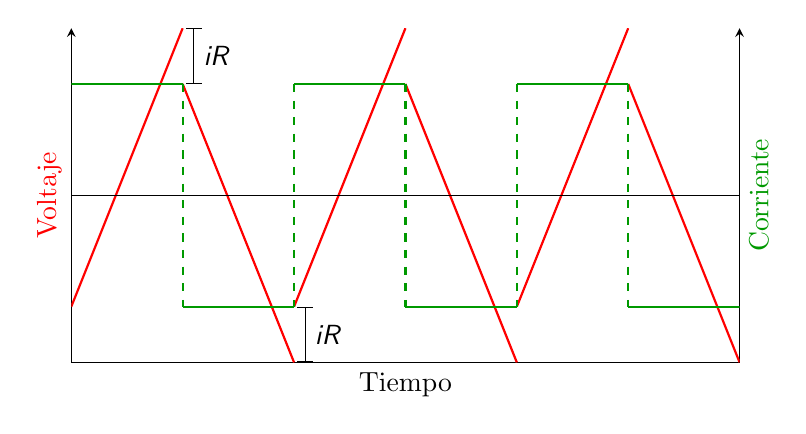
\begin{tikzpicture}
	% let both axes use the same layers
	\pgfplotsset{set layers, 	width=0.7\textwidth, height = 0.35\textwidth}
	
	\begin{axis}[
	scale only axis,
	axis y line=left, % the ’*’ avoids arrow heads
	axis x line*=bottom,
	xlabel=Tiempo,
	ylabel={\color{red} Voltaje},
	no markers,
	xmin=0,
	xmax=6,
	cycle list name=exotic,
	ticks=none,
	]
	\addplot [red, thick] table {
		A B
		%charge
		0 -0.8
		1  1.2
		
		2 -0.8
		3  1.2
		
		4 -0.8
		5  1.2
		
		%discharge
		1  0.8			
		2 -1.2
		
		3  0.8
		4 -1.2
		
		5  0.8
		6 -1.2
	};	
	\draw [arrows={|-|}] (axis cs:1.1,1.2) -- node[right]{$iR$} (axis cs:1.1,0.8);
	\draw [arrows={|-|}] (axis cs:2.1,-1.2) -- node[right]{$iR$} (axis cs:2.1,-0.8);
	\end{axis}
	\begin{axis}[
	scale only axis,
	axis y line=right,
	axis x line=none,
	ylabel={\color{green!60!black} Corriente},
	ymin = -1.5,
	ymax = 1.5,
	xmin = 0,
	xmax = 6,
	no markers,
	ticks=none,
	]
	\addplot [green!60!black, thick] table {
		A B
		0  1
		1  1
		
		1 -1
		2 -1
		
		2  1
		3  1
		
		3 -1
		4 -1
		
		4  1
		5  1
		
		5 -1
		6 -1	
	};
	\addplot [green!60!black, thick, dashed] table {
		A B
		1  1
		1 -1
		
		2  1
		2 -1
		
		3  1
		3 -1
		
		4  1
		4 -1
		
		5  1
		5 -1
	};
	\addplot [black] table {
		0  0
		6  0
	};
	\end{axis}
	\end{tikzpicture}
	\caption[Carga y descarga de un condensador evidenciando el efecto de una ESR]{Carga y descarga de un condensador evidenciando el efecto de una ESR.}
	\label{fig:plot:charge-discharge_esr}
\end{figure}



\subsection{Corriente de fuga (\emph{leakage current})}
Entre los electrodos del condensador fluye una corriente no deseada cuando existe una diferencia de potencial (cuando el condensador está cargado), esta corriente descarga al condensador incluso si está desconectado. Esta imperfección es modelada como una resistencia en paralelo al condensador.

\subsection{Circuito equivalente}
El comportamiento de los condensadores reales (convencionales o electroquímicos), son modelados por un circuito equivalente, donde se introducen componentes que representan las imperfecciones del funcionamiento del condensador real.\\
En la figura \ref{fig:ciruitos_equivalente} se muestran dos circuitos equivalentes empleados para modelar un supercondensador. El de la figura \ref{fig:eq_classic} es un circuito clásico para modelar un supercondensador \citep{Spyker2000}, el de la figura \ref{fig:eq_randles} se denomina circuito Randles, donde el componente adicional marcado con una  letra W, corresponde a la impedancia de Warburg, un elemento que modela la difusión de iones del electrolito \citep{Wang2009}

Con un modelo para el supercondensador, se pueden encontrar los valores para cada componente del circuito equivalente mediante espectroscopia de impedancia electroquímica (EIS).
%\begin{figure}
%	\centering
%	\fbox{
%		\includegraphics[width=0.7\textwidth]{equivalent_both.pdf}
%		}
%	\caption[Circuito equivalente]{Izquierda: Circuito equivalente sencillo. Derecha: Circuito equivalente complejizado \citep{Fletcher2014}.}
%	\label{fig:equiv_both}
%\end{figure}

\newcommand{\circuitscale}{1}
\begin{figure}[h!]
	\centering
	\begin{subfigure}[b]{0.5\textwidth}
		\begin{circuitikz}[scale = \circuitscale, transform shape, font=\large]
			\draw (0,0)
			to [R=$R_s$,  o-] (2,0)
			to [short] (2,-1)
			to [C=$C_{dl}$] (4,-1)
			to [short] (4,0)
			(2,0) to [short] (2,1)
			to [R=$R_{leak}$] (4,1)
			to [short] (4,0)
			to [short, -o] (5,0);
		\end{circuitikz}
		\caption{Circuito equivalente clásico.}
		\label{fig:eq_classic}
	\end{subfigure}\hfill
	\begin{subfigure}[b]{0.5\textwidth}
			\begin{circuitikz}[scale = \circuitscale, transform shape, font=\large]
			\draw (0,0)
			to [R=$R_s$,  o-] (2,0)
			to [short] (2,-1)
			to [R=$R$] (4,-1)
			to [twoport, t=$W$] (6,-1)
			to [short] (6,0)
			(2,0) to [short] (2,1)
			to [C=$C_{dl}$] (6,1)
			to [short] (6,0)
			to [short, -o] (7,0);
			\end{circuitikz}
			\caption{Circuito equivalente Randles.}
			\label{fig:eq_randles}
	\end{subfigure}\\
	\begin{subfigure}{\textwidth}
		\centering
		\begin{tikzpicture}[scale=\plotscale,trim axis right,trim axis left]
		\begin{axis}[
		width=\textwidth,
		height=\axisdefaultheight,
		EISStyle,
		every axis legend/.append style={
			font=\small,
			at={(0.02,0.98)},
			anchor=north west,
		},
		legend entries = {Circuito equivalente clásico, Circuito equivalente Randles}
		]
		\pgfplotstableread{./Data/eisgalv_sim_simple.txt}{\eistable};
		\pgfplotstablegetrowsof{\eistable}
		\pgfmathsetmacro{\N}{\pgfplotsretval}
		\addplot table [only marks, x=Zreal, y expr=\thisrow{Zimag}] {\eistable}
		node[pos=(1-1)/(\N-1), pin=right:{1 MHz}]{}
		node[pos=(\N-1)/(\N-1), pin=right:{0,1 Hz}]{};
		\pgfplotstableread{./Data/eisgalv_sim_warburg.txt}{\eistable};
		\pgfplotstablegetrowsof{\eistable}
		\pgfmathsetmacro{\N}{\pgfplotsretval}
		\addplot table [only marks, x=Zreal, y expr=\thisrow{Zimag}] {\eistable}
		node[pos=(1-1)/(\N-1), pin=left:{1 MHz}]{}
		node[pos=(\N-1)/(\N-1), pin=left:{0,1 Hz}]{};
		\end{axis}
		\end{tikzpicture}
		\label{fig:eis_equivalent}
		\caption[Simulación de circuito equivalente]{Espectro electroquímico de impedancia simulados para los circuitos equivalentes \subref{fig:eq_classic} y \subref{fig:eq_randles}. Obtenido en EIS Spectrum Analyser \footnotemark.}
	\end{subfigure}
	\caption[Circuitos equivalentes]{Circuitos equivalentes.}
	\label{fig:ciruitos_equivalente}
\end{figure}


%%\begin{figure}
%	\centering
%
%%	\begin{circuitikz}[scale =\circuitscale, transform shape]
%%		\draw (1,0)
%%		to [short,o-] (2,0)
%%		to [C=$C_2$] (4,0)
%%		to [R=$R_2$] (6,0)
%%		to [short] (7,0)
%%		(2,0)
%%		to [short] (2,-2)
%%		to [C=$C_1$] (4,-2)
%%		to [R=$R_1$] (6,-2)
%%		to [short] (6,0)
%%		(7,0)
%%		to [short] (7,1)
%%		to [R=$R$] (9,1)
%%		to [short] (9,0)
%%		(7,0)
%%		to [short] (7,-1)
%%		to [C=$C$] (9,-1)
%%		to [short] (9,0)
%%		to [short,-o] (10,0);
%%		\draw[dashed] (2,0)
%%		to [short] (2,3)
%%		(6,3)
%%		to [short] (6,0);
%%		\draw (2,3)
%%		to [C=$C_n$] (4,3)
%%		to [R=$R_n$] (6,3);
%%	\end{circuitikz}
%	\caption{Circuito 1.}
%\end{figure}

\subsection{Supercondensadores}
Un supercondensador es un condensador que exhibe una capacitancia mucho mayor a la de un condensador normal (fácilmente 1000 veces mayor). No utilizan un material dieléctrico, si no un electrolito en cuya interfaz con los electrodos, se forma una doble capa eléctrica. Estos dispositivos están compuestos por dos electrodos de un material de gran área superficial específica, separados por una membrana permeable empapada en electrolito (ver figura \ref{fig:edlc}). Si la capacidad del dispositivo surge de la separación de cargas en una doble capa eléctrica de Helmholtz, se habla de condensadores de doble capa o simplemente supercondensadores. Por otro lado, si la capacitancia surge de reacciones redox en los electrodos, se denominan pseudocondensadores, más aún, si la capacitancia surge de una doble capa y de reacciones redox, se  les llama supercondensadores híbridos, donde generalmente, cada electrodo es de un material diferente y cada uno pensado para un mecanismo distinto de almacenamiento de carga.

\subsection{Doble capa electrostática de Helmholtz}
%TODO explicación doble capa
La gran densidad de energía de un supercondensador tiene que surgir de algún mecanismo de almacenamiento de cargas. A diferencia de las baterías, este mecanismo es puramente físico, pues no hay reacciones químicas en los electrodos, las cargas son separadas en lo que H. Helmholtz llamó \emph{Doble capa electrónica}, (los supercondensadores también son llamados EDLCs, del inglés \emph{Electric Double Layer Capacitors}), la cual consiste en una capa de especies cargadas separadas, a lo largo de la interfaz electrodo-solución\citep{Frackowiak2001}. 
 \footnotetext{Bondarenko A. S., Ragoisha G. A. In Progress in Chemometrics Research, Pomerantsev A. L., Ed.; Nova Science Publishers: New York, 2005, pp. 89–102 (the program is available online at \url{http://www.abc.chemistry.bsu.by/vi/analyser/}}


\begin{figure}[h!]
	\centering
	\fbox{
		\includegraphics[width=0.7\textwidth]{edlc_schem.pdf}
		}
	\caption[Esquema de un supercondensador]{Esquema de un supercondensador mostrando una doble capa eléctrica de Helmholtz en cada electrodo y el perfil del potencial eléctrico en él.}
	\label{fig:edlc}
\end{figure}

\subsection{Pseudocapacitancia}
%TODO
Si, en supercondensador existe intercambio de electrones entre los electrodos y el electrolito (reacciones redox), su densidad de energía aumenta, y por consiguiente surge una capacitancia aparente, que no ha de confundirse con la de un supercondensador de doble capa. El cambio de fase debido a estas reacciones redox, limitan la vida útil y su densidad de energía\citep{Frackowiak2001}. Dicha capacitancia aparente se conoce como pseudocapacitancia y se hace evidente en el gráfico corriente-voltaje en una voltametría cíclica, en forma de picos en potenciales bien definidos.


\subsection{Mediciones en supercondensadores}
Existen varios métodos de caracterización para supercondensadores y dispositivos electroquímicos en general, en este trabajo se utilizarán los tres siguientes: voltametría cíclica, espectroscopia de impedancia electroquímica y ciclos de carga y descarga cíclica.
\subsubsection{Voltametría cíclica}
%TODO explicar mejor
En una voltametría cíclica convencional, se varía el potencial entre los electrodos de manera lineal mientras se mide la corriente. Típicamente el barrido de voltaje se realiza entre dos voltajes fijos, y el recorrido se hace de ida y vuelta. Los parámetros importantes en la voltametría cíclica son: voltajes límite inferior y superior, y velocidad de barrido.

La capacitancia específica $C_s$, puede ser calculada de la voltametría cíclica según la ecuación \ref{eq:cyclic_voltametry},

\begin{equation}\label{eq:cyclic_voltametry}
	C_{s} = \frac{\int_{V_1}^{V_2}i(v) \; dv}{2 \; \Delta V \; m \; \nu },
\end{equation}

donde $i$ y $v$ son la corriente y voltaje instantáneos, $V_1$ y $V_2$ los potenciales límite inferior y superior respectivamente, $\Delta V = V_2 - V_1 $, $m$ es la masa total del material activo en ambos electrodos, y $\nu$ la tasa de barrido. Esta ecuación corresponde a la carga total ($\int i\, dv / \nu$), dividida por la ventana de potencial $\Delta V$ y la masa, el factor $2$ surge de que la voltametría cíclica comprende tanto un ciclo de carga como uno de descarga.

\subsubsection{Espectroscopía de impedancia electroquímica}
Una señal sinusoidal (corriente o voltaje), de determinada amplitud y frecuencia, es aplicada en los terminales del dispositivo midiendo la respuesta de fase y corriente o voltaje según corresponda. La impedancia del sistema es caracterizada en un espectro de frecuencia, el que comúnmente es estudiado entre los mHz y los MHz. Una posible representación de los datos obtenidos es a través del gráfico de Nyquist, el cual consiste en un gráfico paramétrico con la frecuencia como parámetro, donde el eje de las abscisas corresponde a la parte real de la impedancia y las ordenadas a la parte imaginaria. Cualitativamente la forma de la curva obtenida sirve para asignar un circuito equivalente al dispositivo estudiado, sin embargo, también es posible calcular algunas cantidades, como por ejemplo la resistencia en serie equivalente.

\subsubsection{Carga y descarga cíclica}
En este proceso la corriente es aplicada de forma constante para cargar el condensador hasta un potencial preestablecido, cuando dicho potencial es alcanzado, se aplica una corriente en sentido contrario para descargar el condensador hasta un potencial inferior predefinido. Generalmente, la corriente de carga y descarga son de igual magnitud. De las curvas de carga y descarga se puede determinar la capacitancia del condensador, y la resistencia en serie equivalente. Extendiendo la medición a miles de ciclos (hasta 10.000 ciclos), se puede determinar cómo será el comportamiento del dispositivo al pasar el tiempo.
\part{Cuerpo de la tesis}
\chapter{Síntesis de óxido de grafeno}
\chapter{Reducción del óxido de grafeno}
\chapter{Construcción de supercondensadores}
\chapter{Conclusiones}
%\addcontentsline{toc}{chapter}{Conclusiones}
En este trabajo de tesis se implementó un método efectivo para medir el desempeño de materiales basados en carbono como electrodos de supercondensadores, que resultó ser apropiado para determinar diferencias en la construcción de los electrodos. Además, se sintetizó un material de carbono para ser utilizado como electrodo en dichos condensadores.
%\appendix
\chapter*{Anexo}
\addcontentsline{toc}{chapter}{Anexo}
\section{Caracterización electroquímica}

\SCGraphsNoMass{CV_Steel_Disk_No_Material_1}{CV_Steel_Disk_No_Material_2}{0}{16}{1954.91833300000}{Disco de acero sin material.}{200}
\SCGraphs{CV_CRGO300517_9}{CV_CRGO300517_10}{0.0004}{10}{3101.89233300000}{Polvo en disco de acero. Masa = 0.4 mg.}{0.0002}
\SCGraphs{CV_CRGO300517_3}{CV_CRGO300517_4}{0.0028}{20}{2105.33533300000}{Polvo + PMMA en disco de acero. Masa = 2.8 mg.}{0.0002}
\SCGraphs{CV_CRGO300517_11}{CV_CRGO300517_12}{0.0006}{250}{45656.2866670000}{Papel en disco de acero. Masa = 0.6 mg.}{0.0001}
\SCGraphs{CV_CRGO300517_13}{CV_CRGO300517_14}{0.0006}{465}{86333.0367000000}{Material liofilizado en disco de acero. Masa = 0.6 mg.}{0.0001}

\SCGraphsNoMass{CV_Nickel_Foam_No_Material_1}{CV_Nickel_Foam_No_Material_2}{0}{12}{2399.28233300000}{Espuma de níquel sin material.}{200}
\SCGraphs{CV_CRGO300517_5}{CV_CRGO300517_6}{0.0009}{12}{4328.46733300000}{Polvo en espuma de níquel. Masa = 0.9 mg.}{0.0002}
\SCGraphs{CV_CRGO300517_7}{CV_CRGO300517_8}{0.0008}{5}{771.593133000000}{Polvo + PMMA en espuma de níquel. Masa = 0.8 mg.}{0.0002}

%%ÍNDICE ANALÍTICO
%\newpage
%\printindex
%\addcontentsline{toc}{chapter}{Índice Analítico}

%%BIBLIOGRAFÍA
\newpage

\bibliography{Nanosintesis}
\bibliographystyle{apalike}

\end{document}